\documentclass[11pt, english, fleqn, DIV=15, headinclude, BCOR=2cm]{scrreprt}

\usepackage[
    color,
    bibatend,
]{../../header}

\graphicspath{{_build/}{../Figures/}}

\newcommand\MZ{M_{\mathrm Z^0}}

\usepackage{mathtools}

\hypersetup{
    pdftitle=
}

\usepackage{longtable}
\usepackage{subcaption}

\usepackage[all]{nowidow}

\subject{Lab report}
\title{Analysis of $Z_0$ decays}
\subtitle{Experiment K213 -- Universität Bonn}
\author{%
    Martin Ueding \\
    \small{\href{mailto:mu@martin-ueding.de}{mu@martin-ueding.de}}
    \and
    Lino Lemmer \\
    \small{\href{mailto:l2@uni-bonn.de}{l2@uni-bonn.de}}
}

\date{2016-03-02}

\publishers{Tutor: David Hohn}

\begin{document}

\maketitle

\begin{abstract}
\end{abstract}

\tableofcontents

\chapter*{Permission to upload}

I, Martin Ueding, would like to scan and upload this lab report with your
corrections to my website \href{http://martin-ueding.de}{martin-ueding.de}.
There, the original lab report as well as the reviewed one will be licensed
under the “\href{http://creativecommons.org/licenses/by-sa/4.0/}{Creative
Commons Attribution-ShareAlike 4.0 International License}”. Is that okay with
you?

Yes $\Box$ \hspace{2cm} No $\Box$

\chapter{Theory}

\begin{figure}
    \centering
    \includegraphics{radiative_interpolation}
    \caption{%
        Radiation corrections given in the experiment description on page~4. We
        have interpolated with quadratic splines.
    }
    \label{fig:radiative_interpolation}
\end{figure}

\chapter{Exercises}

There are a couple of exercises that are supposed to be done before the
experiment.

\section{Decay width}

We are to compute the decay width~$\Gamma$ of a $\mathrm Z^0$ particle into a
pair of various fermions. The top-quark is heavier than the gauge boson,
therefore it cannot decay into a pair of top-quarks. The Feynman diagram
corresponding to the decay is shown in Figure~\ref{fig:z0-decay}.

\begin{figure}
    \centering
    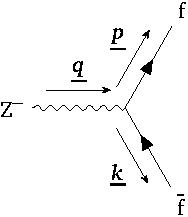
\includegraphics{z0-decay}
    \caption{%
        Decay of a $\mathrm Z^0$ gauge boson into a pair of fermions. Time is
        to the right.
    }
    \label{fig:z0-decay}
\end{figure}

First we compute the invariant matrix element~$\mathcal M$. Reading off the
Feynman diagram, we have
\begin{align*}
    \iup \mathcal M
    &= \epsilon^\mu \bar u^s(\four p) \frac{\iup g}{\cos(\theta_\text w)}
    \mat\gamma_\mu \del{g_\text v^f - g_\text a^f \mat\gamma_5} v^{s'}(\four k)
    \,,
    \intertext{%
        where we have used the rules given by \textcite[(D.56)]{romao/aqt}. We
        chose the center of mass system, as we always can for a single massive
        particle, and have $\four q = (\sqrt s, \vec 0)$. As the gauge boson
        does not have any three momentum direction, we can choose the
        polarization vector $\four \epsilon$ like we want. We chose it in the
        positive $x^3$-direction and have $\four \epsilon = (0, 0, 0, 1)$. With
        that we can simplify the Lorentz structure a little bit and obtain
    }
    &= \bar u^s(\four p) \frac{\iup g}{\cos(\theta_\text w)}
    \mat\gamma_3 \del{g_\text v^f - g_\text a^f \mat\gamma_5} v^{s'}(\four k)
    \,.
\end{align*}

For the decay width, which we are interested in, we need the modulus squared of
the matrix element. For that we need the following:
\begin{multline*}
    \sbr{\bar u^s(\four p) \mat\gamma_3 \del{g_\text v^f - g_\text a^f \mat\gamma_5}
    v^{s'}(\four k)}^\dagger \\
    =
    v^{s'}(\four k)^\dagger
    \del{g_\text v^f - g_\text a^f \mat\gamma_5^\dagger}
    \mat\gamma_3^\dagger
    \mat\gamma_0
    u^s(\four p) \\
    =
    \underbracket{v^{s'}(\four k)^\dagger
    \mat\gamma_0}
    \underbracket{\mat\gamma_0
        \del{g_\text v^f - g_\text a^f \mat\gamma_5^\dagger}
    \mat\gamma_0}
    \underbracket{\mat\gamma_0
        \mat\gamma_3^\dagger
    \mat\gamma_0}
    u^s(\four p) \\
    = \bar v^{s'}(\four k)
    \del{g_\text v^f + g_\text a^f \mat\gamma_5}
    \mat\gamma_3
    u^s(\four p) \\
    = \bar v^{s'}(\four k)
    \mat\gamma_3
    \del{g_\text v^f - g_\text a^f \mat\gamma_5}
    u^s(\four p) \,. \\
\end{multline*}

Now we can write the modulus squared of the matrix element
\begin{align*}
    |\mathcal M|^2
    &= \frac{g^2}{\cos(\theta_\text w)^2}
    \bar v^{s'}(\four k)
    \mat\gamma_3
    \del{g_\text v^f - g_\text a^f \mat\gamma_5}
    u^s(\four p)
    \bar u^s(\four p)
    \mat\gamma_3
    \del{g_\text v^f - g_\text a^f \mat\gamma_5}
    v^{s'}(\four k)
    \,. \\
    \intertext{%
        As the detector is not sensitive to the spin of the resulting fermions,
        we need to sum over all the final state spin configurations $s$ and
        $s'$. This will give us a fermion trace,
    }
    \sum_\text{spins} |\mathcal M|^2
    &=
    \frac{g^2}{\cos(\theta_\text w)^2}
    \tr\del{
        \four k
        \mat\gamma_3
        \del{g_\text v^f - g_\text a^f \mat\gamma_5}
        \four p
        \mat\gamma_3
        \del{g_\text v^f - g_\text a^f \mat\gamma_5}
    }
    \,, \\
    \intertext{%
        where we have neglected the masses of the fermions. The second
        parentheses with $\mat\gamma_5$ can be anticommuted twice and be
        collapsed with the first one. We have
    }
    &=
    \frac{g^2}{\cos(\theta_\text w)^2}
    \tr\del{
        \four k
        \mat\gamma_3
        \del{g_\text v^f - g_\text a^f \mat\gamma_5}^2
        \four p
        \mat\gamma_3
    }
    \,, \\
    \intertext{%
        where we can now simplify this. As an aside, we have
        \[
            \del{g_\text v^f - g_\text a^f \mat\gamma_5}^2
            = (g_\text v^f)^2 - (g_\text a^f)^2 - 2 g_\text v^f g_\text a^f
            \mat\gamma_5 \,.
        \]
        The square of $\mat\gamma_5$ is just the unit matrix in Dirac space.
        The term with $\mat\gamma_5$ will drop out as the trace identity
        contains the Levi-Civita symbol~$\epsilon_{\mu\nu\rho\gamma}$ which
        will be zero if two of the indices are 3, as we have in our case.
        Therefore we can directly drop that term. As it does not contain any
        further Dirac structure, we can pull it out front and obtain
    }
    &=
    \frac{g^2}{\cos(\theta_\text w)^2}
    \del{(g_\text v^f)^2 - (g_\text a^f)^2}
    \tr\del{
        \four k
        \mat\gamma_3
        \four p
        \mat\gamma_3
    }
    \,.
    \intertext{%
        Using a trace identity like given by \textcite[(A.27)]{Peskin/QFT/1995}
        we obtain
    }
    &= \frac{4 g^2}{\cos(\theta_\text w)^2} \del{(g_\text v^f)^2 - (g_\text a^f)^2}
    (2 k_3 p_3 + \four k \cdot \four p) \,.
\end{align*}
This is our final form of the matrix element.

The decay width is given by additional factors and a integration over phase
space. We have
\begin{align*}
    \Gamma_f
    &= \frac{1}{2 M_{\mathrm Z^0}} (2 \piup)^4 \int
    \frac{\dif^3 p}{(2\piup)^3 2 E_{\vec p}}
    \frac{\dif^3 k}{(2\piup)^3 2 E_{\vec k}}
    \delta^4(\four q - \four k - \four p)
    |\mathcal M|^2 \,.
    \intertext{%
        We simplify the factors and insert the matrix element and get
    }
    &= \frac{1}{32 \piup^2 M_{\mathrm Z^0}} \int
    \frac{\dif^3 p}{E_{\vec p}}
    \frac{\dif^3 k}{E_{\vec k}}
    \delta^4(\four q - \four k - \four p)
    \frac{4 g^2}{\cos(\theta_\text w)^2}
    \del{(g_\text v^f)^2 - (g_\text a^f)^2}
    (2 k_3 p_3 + \four k \cdot \four p) \,.
    \intertext{%
        Then we simplify even more and obtain
    }
    &= \frac{1}{8 \piup^2 M_{\mathrm Z^0}}
    \frac{g^2}{\cos(\theta_\text w)^2}
    \del{(g_\text v^f)^2 - (g_\text a^f)^2}
    \int
    \frac{\dif^3 p}{E_{\vec p}}
    \frac{\dif^3 k}{E_{\vec k}}
    \delta^4(\four q - \four k - \four p)
    (2 k_3 p_3 + \four k \cdot \four p) \,.
    \intertext{%
        The total energy-momentum conserving Dirac-distribution can be split
        into time-like and space-like part. In the center-of-mass frame, this
        gives us
    }
    &= \frac{1}{8 \piup^2 M_{\mathrm Z^0}}
    \frac{g^2}{\cos(\theta_\text w)^2}
    \del{(g_\text v^f)^2 - (g_\text a^f)^2}
    \\&\qquad\times
    \int
    \frac{\dif^3 p}{E_{\vec p}}
    \frac{\dif^3 k}{E_{\vec k}}
    \delta(\sqrt s - E_{\four k} - E_{\four p})
    \delta^3(\vec k + \vec p)
    (2 k_3 p_3 + \four k \cdot \four p) \,,
    \intertext{%
        which suggests the following change in variables:
        \[
            \vec a := \vec p + \vec k
            \eqnsep
            \vec b := \frac{\vec p - \vec k}{2} \,.
        \]
        The Jacobian of this transformation is unity. The $\delta^3(\vec k +
        \vec p)$ will become $\delta^3(\vec a)$, in the $\int \dif^3 a$
        integral, this will set $\vec a$ to $\vec 0$. So far we have
    }
    &= \frac{1}{8 \piup^2 M_{\mathrm Z^0}}
    \frac{g^2}{\cos(\theta_\text w)^2}
    \del{(g_\text v^f)^2 - (g_\text a^f)^2}
    \int
    \frac{\dif^3 b}{E_{\vec p} E_{\vec k}}
    \delta(\sqrt s - E_{\vec k} - E_{\vec p})
    (2 k_3 p_3 + \four k \cdot \four p) \,.
    \intertext{%
        Now we have to replace $k$ and $p$ with $b$. We have $\vec p = \vec b$
        and $\vec k = - \vec b$. Their magnitude is the same, which is expected
        in the center-of-mass frame in a two body decay. This simplifies the
        relations to
    }
    &= \frac{1}{8 \piup^2 M_{\mathrm Z^0}}
    \frac{g^2}{\cos(\theta_\text w)^2}
    \del{(g_\text v^f)^2 - (g_\text a^f)^2}
    \int
    \frac{\dif^3 b}{E_{\vec b}^2}
    \delta(\sqrt s - 2 E_{\vec b})
    (- 2 b_3 b_3 + E_{\vec b}^2 + \vec b \cdot \vec b) \,.
    \intertext{%
        As we have massless particles, we have $E_{\vec b} = |\vec b|$. We
        change into spherical coordinates in $\vec b$ and obtain
    }
    &= \frac{1}{4 \piup M_{\mathrm Z^0}}
    \frac{g^2}{\cos(\theta_\text w)^2}
    \del{(g_\text v^f)^2 - (g_\text a^f)^2}
    \\&\qquad\times
    \int \dif b \, b^2 \int \dif \cos(\theta) \,
    \frac{1}{b^2}
    \delta(\sqrt s - 2 b)
    (- 2 b^2 \cos(\theta)^2 + b^2 + b^2) \,,
    \intertext{%
        where we have performed $\int \dif \phi = 2 \piup$ already as we do not
        have any explicit $\phi$-dependence. The radial integration will set $b
        = \sqrt s / 2$. In our case $s = M_{\mathrm Z^0}^2$ and we have
    }
    &= \frac{M_{\mathrm Z^0}}{16 \piup}
    \frac{g^2}{\cos(\theta_\text w)^2}
    \del{(g_\text v^f)^2 - (g_\text a^f)^2}
    \int \dif \cos(\theta) \,
    (- 2 \cos(\theta)^2 + 2) \,.
    \intertext{%
        The angular integration gives $(-4/3 + 4) = 8/3$, so we get
    }
    &= \frac{M_{\mathrm Z^0}}{6 \piup}
    \frac{g^2}{\cos(\theta_\text w)^2}
    \del{(g_\text v^f)^2 - (g_\text a^f)^2} \,.
    \intertext{%
        Replacing $g^2$ with $8 M_{\mathrm Z^0}^2 G_\text F / \sqrt 2$, we will
        obtain
    }
    &= \frac{4}{3 \piup \sqrt 2}
    \frac{G_\text F M_{\mathrm Z^0}^3}{\cos(\theta_\text w)^2}
    \del{(g_\text v^f)^2 - (g_\text a^f)^2} \,.
\end{align*}

Except for factors up front, this is the same as Equation~(2.12) given in the
manual.

% FIXME Find the missing factors.

We can now insert the various quantum numbers of particles, insert the numbers
and obtain the decay widths. Our results are listed in
Table~\ref{tab:decay_widths}.

The Fermi coupling constant has the value \SI{<< fermi_coupling
>>}{\per\giga\electronvolt\squared}.
% TODO Cite PDG.

\begin{table}
    \centering
    \begin{tabular}{lcccS}
        \toprule
        Flavor & $I_3$ & $Q$ & $N_\text c$ & $\Gamma / \si{\mega\electronvolt}$ \\
        \midrule
        Electron & $-1/2$ & $-1$ & 1 & << gamma_electron >> \\
        Neutrino & $1/2$ & $0$ & 1 & << gamma_neutrino >> \\
        Up-Quark & $1/2$ & $2/3$ & 3 & << gamma_up_type >> \\
        Down-Quark & $-1/2$ & $-1/3$ & 3 & << gamma_down_type >> \\
        \bottomrule
    \end{tabular}
    \caption{%
        Decay widths for the various families of fermions. As the fermions are
        taken to be massless, only one representative of the family is
        mentioned in the column \enquote{Flavor}.
    }
    \label{tab:decay_widths}
\end{table}

\section{Partial widths}

In the previous section, we have computed the decay widths for each kind of
particle. Now we have to group the various particles into families and add
their partial widths.

\begin{description}
    \item[Hadronic width]
        The hadrons in the final state are the up, down, strange, charm and
        bottom quarks. Therefore we have two up-type and three down-type quarks
        which results in a width of
        $\Gamma_\text{had.} = \SI{<< hadronic_width >>}{\mega\electronvolt}$.
        The branching ratio here is \num{<< hadronic_ratio >>}.

    \item[Charged leptonic width]
        The charged leptons are the electron, the myon and the tau. The charged
        leptonic width therefore is
        $\Gamma_\text{ch.lep.} = \SI{<< charged_leptonic_width >>}{\mega\electronvolt}$.
        The branching ratio here is \num{<< charged_leptonic_ratio >>}.

    \item[Neutral leptonic width]
        The neutral leptons are the electron-neutrino, the myon-neutrino and
        the tau-neutrino. The neutral
        leptonic width therefore is
        $\Gamma_\text{n.lep.} = \SI{<< neutral_leptonic_width >>}{\mega\electronvolt}$.
        The branching ratio here is \num{<< neutral_leptonic_ratio >>}.

    \item[Total width]
        Summing all those widths up, we obtain
        $\Gamma_\text{tot.} = \SI{<< total_width >>}{\mega\electronvolt}$.
\end{description}

All numerical values as well as the partial cross sections are in
Table~\ref{tab:partial_stuff}. The total cross section is
\[
    \sigma_\text{total}^\text{peak} = \frac{12 \piup}{\MZ^2} \frac{\Gamma_\text
    e}{\Gamma_{\mathrm Z^0}} \,.
\]

\begin{table}
    \centering
    \begin{tabular}{lSSS}
        \toprule
        Type & {Width / \si{\mega\electronvolt}} & {Branching ratio} & {Partial
    cross section / \SI{e-11}{\per\mega\electronvolt\squared}} \\
        \midrule
        Hadronic
        & << hadronic_width >> & << hadronic_ratio >> & <<
        hadronic_partial_cross_section >> \\
        Charged leptonic
        & << charged_leptonic_width >> & << charged_leptonic_ratio >> & <<
        charged_leptonic_partial_cross_section >> \\
        Neutral leptonic
        & << neutral_leptonic_width >> & << neutral_leptonic_ratio >> & <<
        neutral_leptonic_partial_cross_section >> \\
        Total
        & << total_width >> & 1 & <<
        total_cross_section >> \\
        \bottomrule
    \end{tabular}
    \caption{%
        Partial decay widths, branching ratios and cross sections.
    }
    \label{tab:partial_stuff}
\end{table}

%%%%%%%%%%%%%%%%%%%%%%%%%%%%%%%%%%%%%%%%%%%%%%%%%%%%%%%%%%%%%%%%%%%%%%%%%%%%%%%

\end{document}

% vim: spell spelllang=en_us tw=79
